\documentclass[10pt]{beamer}

\usetheme{metropolis}
\usepackage{appendixnumberbeamer}

\usepackage{booktabs}
\usepackage[scale=2]{ccicons}

\usepackage{listings}

\usepackage{xspace}
\newcommand{\themename}{\textbf{\textsc{metropolis}}\xspace}

\title[RnD Summit Talk 2016]{Revisiting The Art of Computer Programming}
\date{\today}
\author{Andreas Bok Andersen}

\usepackage[doi=false,isbn=false,url=false,style=numeric]{biblatex}
\addbibresource{Remote.bib}
\setbeamercovered{transparent}
\begin{document}

\maketitle

% \section{Knuth - A very very short introduction}

\begin{frame}
  \frametitle{Knuth - A very short introduction}
  \begin{columns}[c]
    \column{0.4\textwidth}
        \includegraphics<-2>[width=0.9\textwidth]{./media/Knuth-A-small.jpg}
        \includegraphics<3>[width=0.9\textwidth]{./media/Knuth-B-small.jpg}
        \includegraphics<4>[width=0.9\textwidth]{./media/dek-14May10-1.jpeg}
        \includegraphics<5->[width=0.9\textwidth]{./media/dek-14May10-2-cropped.jpeg}
    \column{0.6\textwidth}
        \begin{itemize}[<+->]
          \item Donald Ervin Knuth (1938-)
          \item Stanford University (1968-)
          \item TAOCP (1968-)
          \item ACM Turing Award (1974)
          \item \TeX \phantom{a} (1978)
          \item Thrice in XKCD, \href{https://xkcd.com/163}{163}, \href{https://xkcd.com/342}{342}, \href{https://xkcd.com/816}{816}
        \end{itemize}
  \end{columns}
\end{frame}
\cite{}
\begin{frame}[fragile]
  \frametitle{The Art of Computer Programming (TAOCP)}
  \begin{block}{The Art of Computer Programming (TAOCP)\\Volumes 1-7\\}
    \begin{itemize}
          \item[] 1 – Fundamental Algorithms (1968)
          \item[] 2 – Seminumerical Algorithms (1969)
          \item[] 3 – Sorting and Searching (1973)
          \item[]<2-> 4 – Combinatorial Algorithms (2005-2015)
          \item[]<3-> 5 – Syntactic Algorithms (as of 2015, estimated for release in 2025)
          \item[]<3-> 6 – The Theory of Context-Free Languages (planned)
          \item[]<3-> 7 – Compiler Techniques (planned)
    \end{itemize}
  \end{block}
\end{frame}

\begin{frame}
  \frametitle{The Art of Computer Programming (TAOCP)}
  \begin{columns}[c]
    \column{0.3\textwidth}
      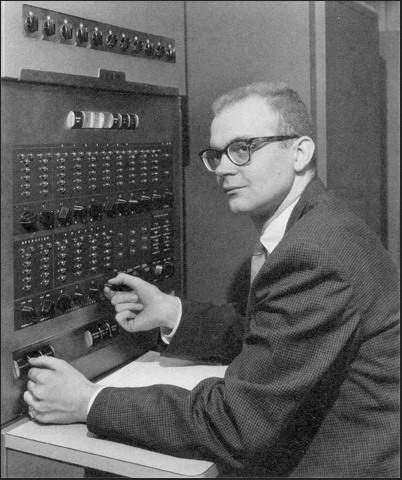
\includegraphics[width=1\textwidth]{./media/Don-Knuth-ibm-650-1958.jpg}
    \column{0.7\textwidth}
        \begin{quote}
This series of books is affectionately dedicated to the Type 650 computer once installed at Case Institute of Technology, in remembrance of many pleasant evenings.\cite{Knuth1973Art}
        \end{quote}

  \end{columns}
   \note[itemize]{
    \item Contrast with how Knuth put the Science into Computer Science
    \item  citation: major contributions to the analysis of algorithms and the design of programming languages, and in particular for his contributions to the TAOCP, science
  }
\end{frame}

% \section{Art, Creativity and Programming}

\begin{frame}[fragile]
  \frametitle{Knuth's sense of Art}
  \begin{block}{ACM Award Lecture}
    \begin{quote}
    The process of preparing programs for a digital computer is especially attractive, not only because it can be economically and scientifically rewarding, but also because it can be an \textbf{aesthetic experience much like composing poetry or music}. [emphasis added]\cite[v]{Knuth1973Art}
    \end{quote}

  \begin{quote}<2->
    ...computer programming is an art, because it applies accumulated knowledge to the world, because it requires skill and ingenuity, and especially because it produces \textbf{objects of beauty}.\cite{Knuth1974Computer}
  \end{quote}
  \end{block}
\end{frame}

\begin{frame}
  \frametitle{Creativity and the brain}
  \begin{center}
    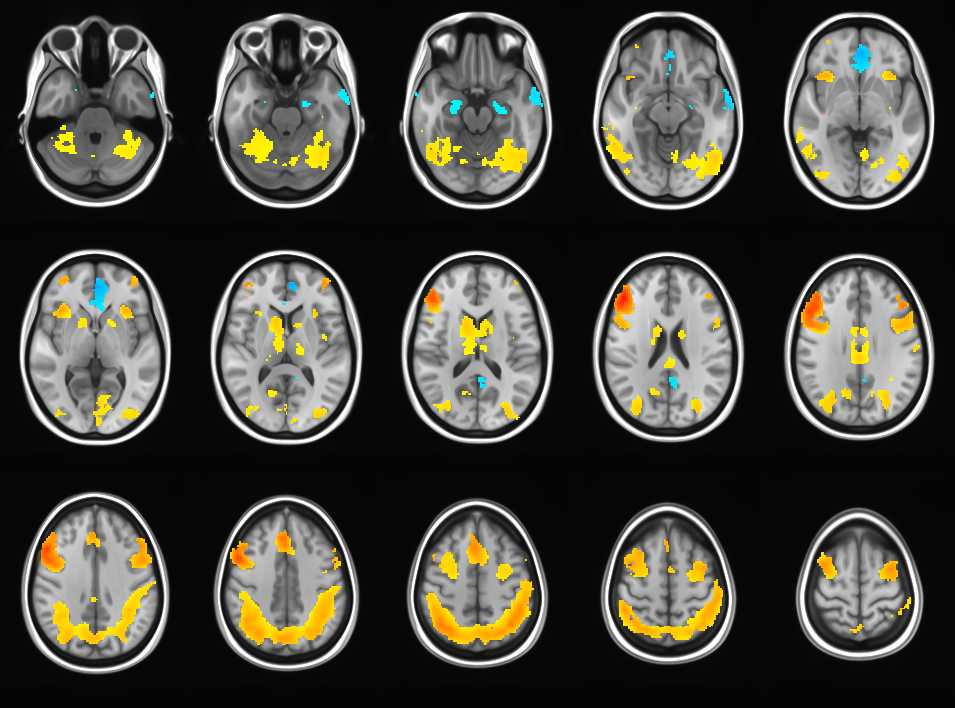
\includegraphics[height=0.75\textheight]{./media/fmri-example.png}
  \end{center}
\end{frame}

\begin{frame}
  \frametitle{Neural plasticity - We are what we do}
  \begin{itemize}[<+->]
    \item Neural Pathways in the brain are continuously reorganized by what we learn and experience
    \item Our professional and personal lives are reflected in the brain
  \end{itemize}
\end{frame}

\begin{frame}
  \frametitle{We are what we do}
  {
  \only<1>{
    \begin{block}{London Bus versus Taxi Drivers}
      \begin{quote}
      Experienced London taxi drivers have larger parahippocampal regions with size correlated with years of experience.\cite{Maguire2006London}
      \end{quote}
      \begin{quote}
      the ability to acquire new visuospatial information was worse in taxi drivers than in bus drivers\cite{Maguire2006London}
      \end{quote}

    \end{block}}
  }

  {
  \only<2>{\begin{block}{Professional Video Gamers}
    \begin{quote}
    ...significantly larger gray matter volume in the right posterior parietal cortex in experts[video game players] compared with non-experts\cite{Tanaka2013Larger}
    \end{quote}
  \end{block}}
  }

  {
  \only<3>{\begin{block}{Musicians vs. Non-Musicians}
    \begin{quote}
      Perception of rhythm and meter is significantly different in musicians vs. non-musicians
     \cite{Vuust2012Practiced},\cite{Vuust2011Tapping}
     \end{quote}
  \end{block}}
  }
\end{frame}

\begin{frame}
  \frametitle{Neuroscience of programming (Siegmund et. al. 2014)}
  \begin{block}{Understanding understanding source code}
    \begin{itemize}[<+->]
      \item First (and so far only) study of computer programmers' brains using functional Magnetic Resonance Imaging (fMRI)
      \item Comprehension of source code snippets (Factorial, Find largest in list of numbers)
      \item \textit{programming} had less in common with mathematics and more in common with language
    \end{itemize}
  \end{block}

\end{frame}

\begin{frame}
  \frametitle{Neuroscience of programming (Siegmund et. al. 2014)}
  \begin{columns}[c]
    \column{0.5\textwidth}
      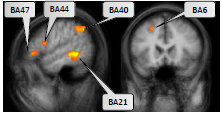
\includegraphics[width=0.9\textwidth]{./media/92170_Figure1-cropped.png}
    \column{0.5\textwidth}
      \only<2->{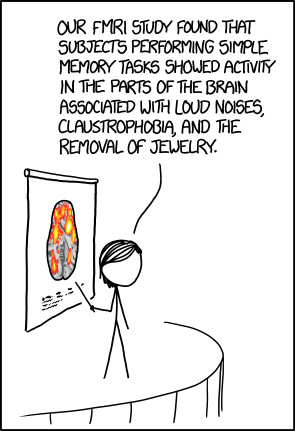
\includegraphics[width=.8\textwidth]{./media/xkcd-fmri.png}}
  \end{columns}

  \note{
    Comparative study of subjects with and without a computer science background
  }
\end{frame}

\begin{frame}
  \frametitle{Sooooooo}
  \begin{itemize}
    \item
  \end{itemize}
\end{frame}

\begin{frame}[standout]
  Questions?
\end{frame}

\appendix

\begin{frame}[allowframebreaks]{References}
  \printbibliography

\end{frame}

\end{document}
